\documentclass{article}
\usepackage[utf8]{inputenc}
\usepackage[hungarian]{babel}

\usepackage{lipsum}
\usepackage{graphicx} % for the includegrapichs
\usepackage{titling}

\usepackage{fancyhdr} % for the header on the first page
\usepackage{pdfpages} % to include pdf
\usepackage{structuralanalysis} % for the figures



\begin{document}
	
	\begin{titlepage}
		\setlength{\headheight}{20pt}
		\lhead{
\includegraphics[height=1.5cm]{logo_mm.png}}
		\rhead{\large{\textbf{Végeselem módszer alapjai}}\\
			BMEGEMMAGMV}
		%\vspace{15cm}
		\title{\huge Kötelező házi feladat 1
		}
		\author{Tar Dániel\\GUTOY7}
		\date{\today}
		\maketitle
		\pagenumbering{gobble}
		\thispagestyle{fancy}
		
		\begin{figure}
			\begin{center}
				
\includegraphics[height=2cm]{logo_bme_kicsi.eps}
			\end{center}
		\end{figure}
		
	\end{titlepage}
	\newpage

	%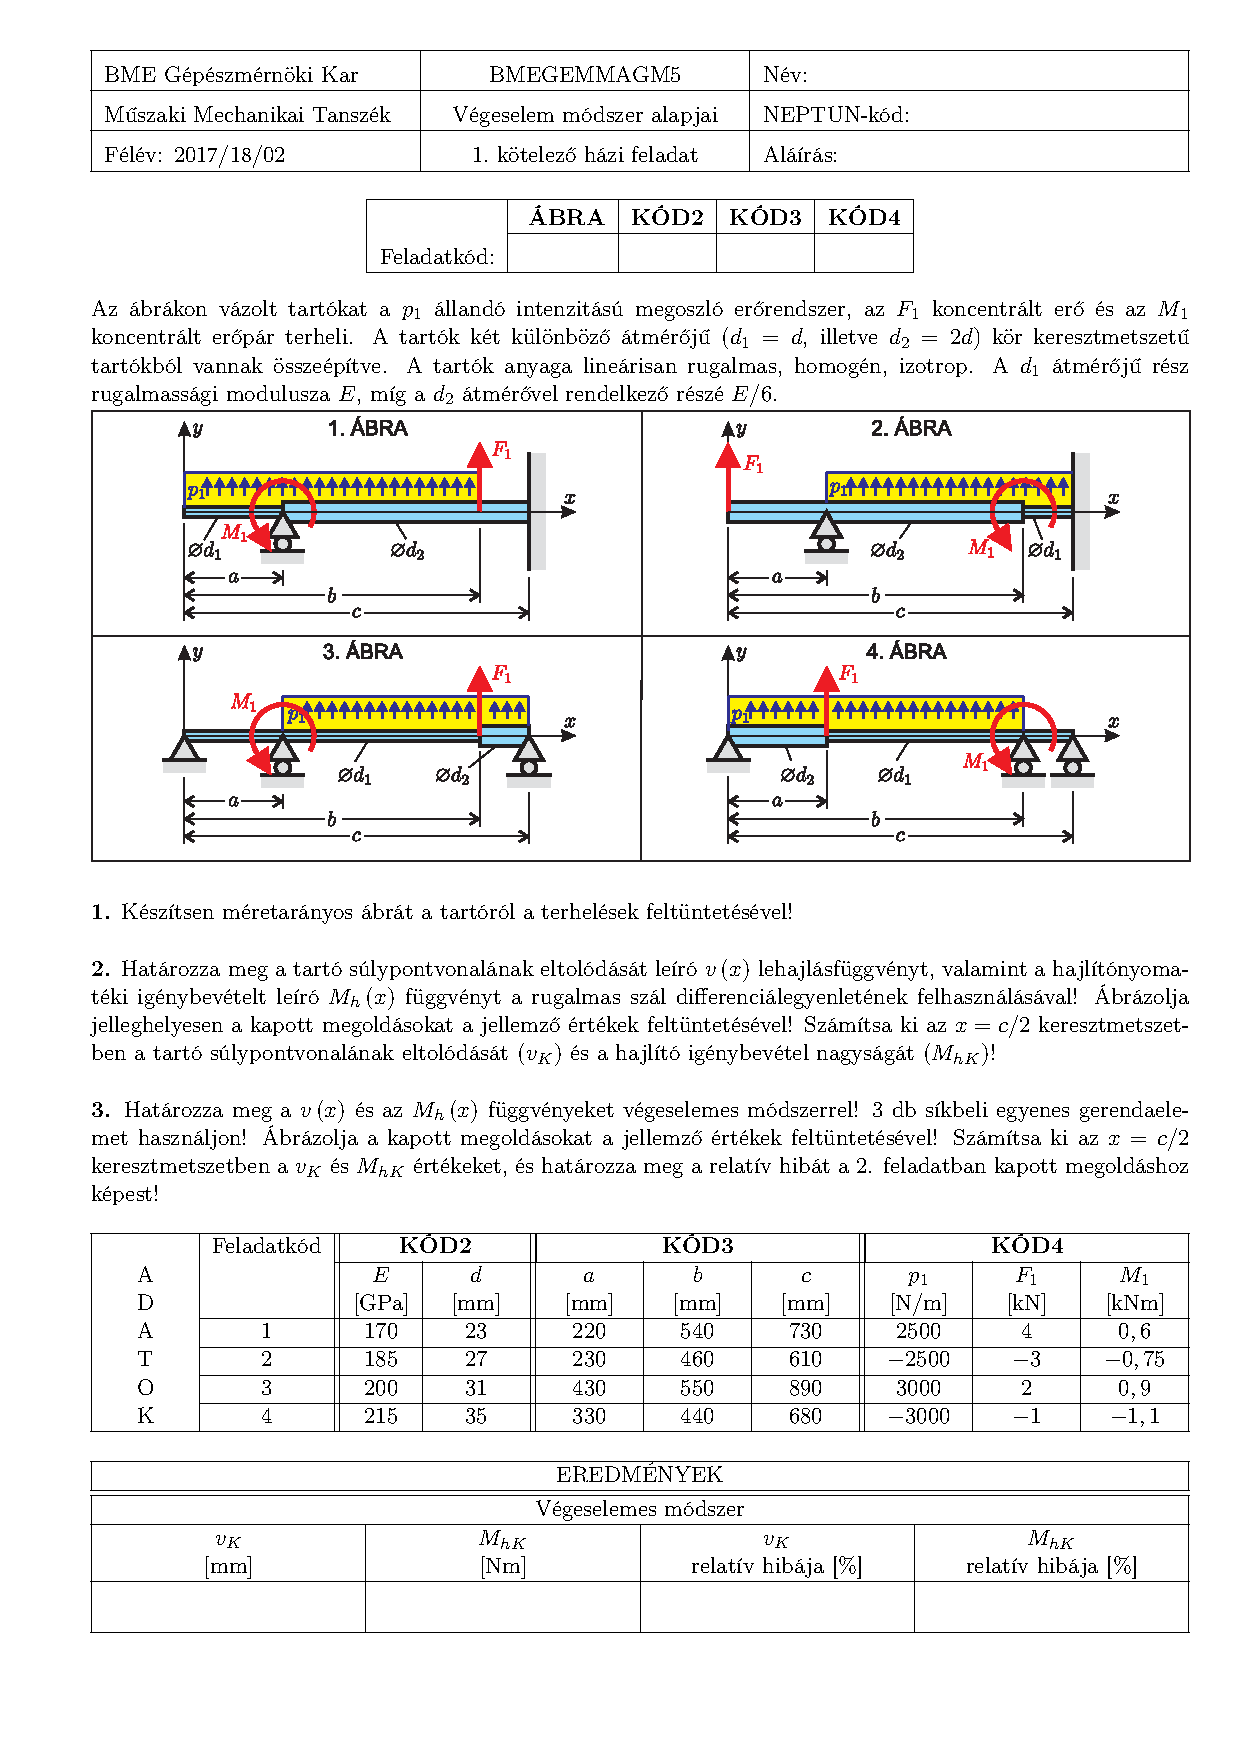
\includepdf{vemalaphf1.pdf}
	 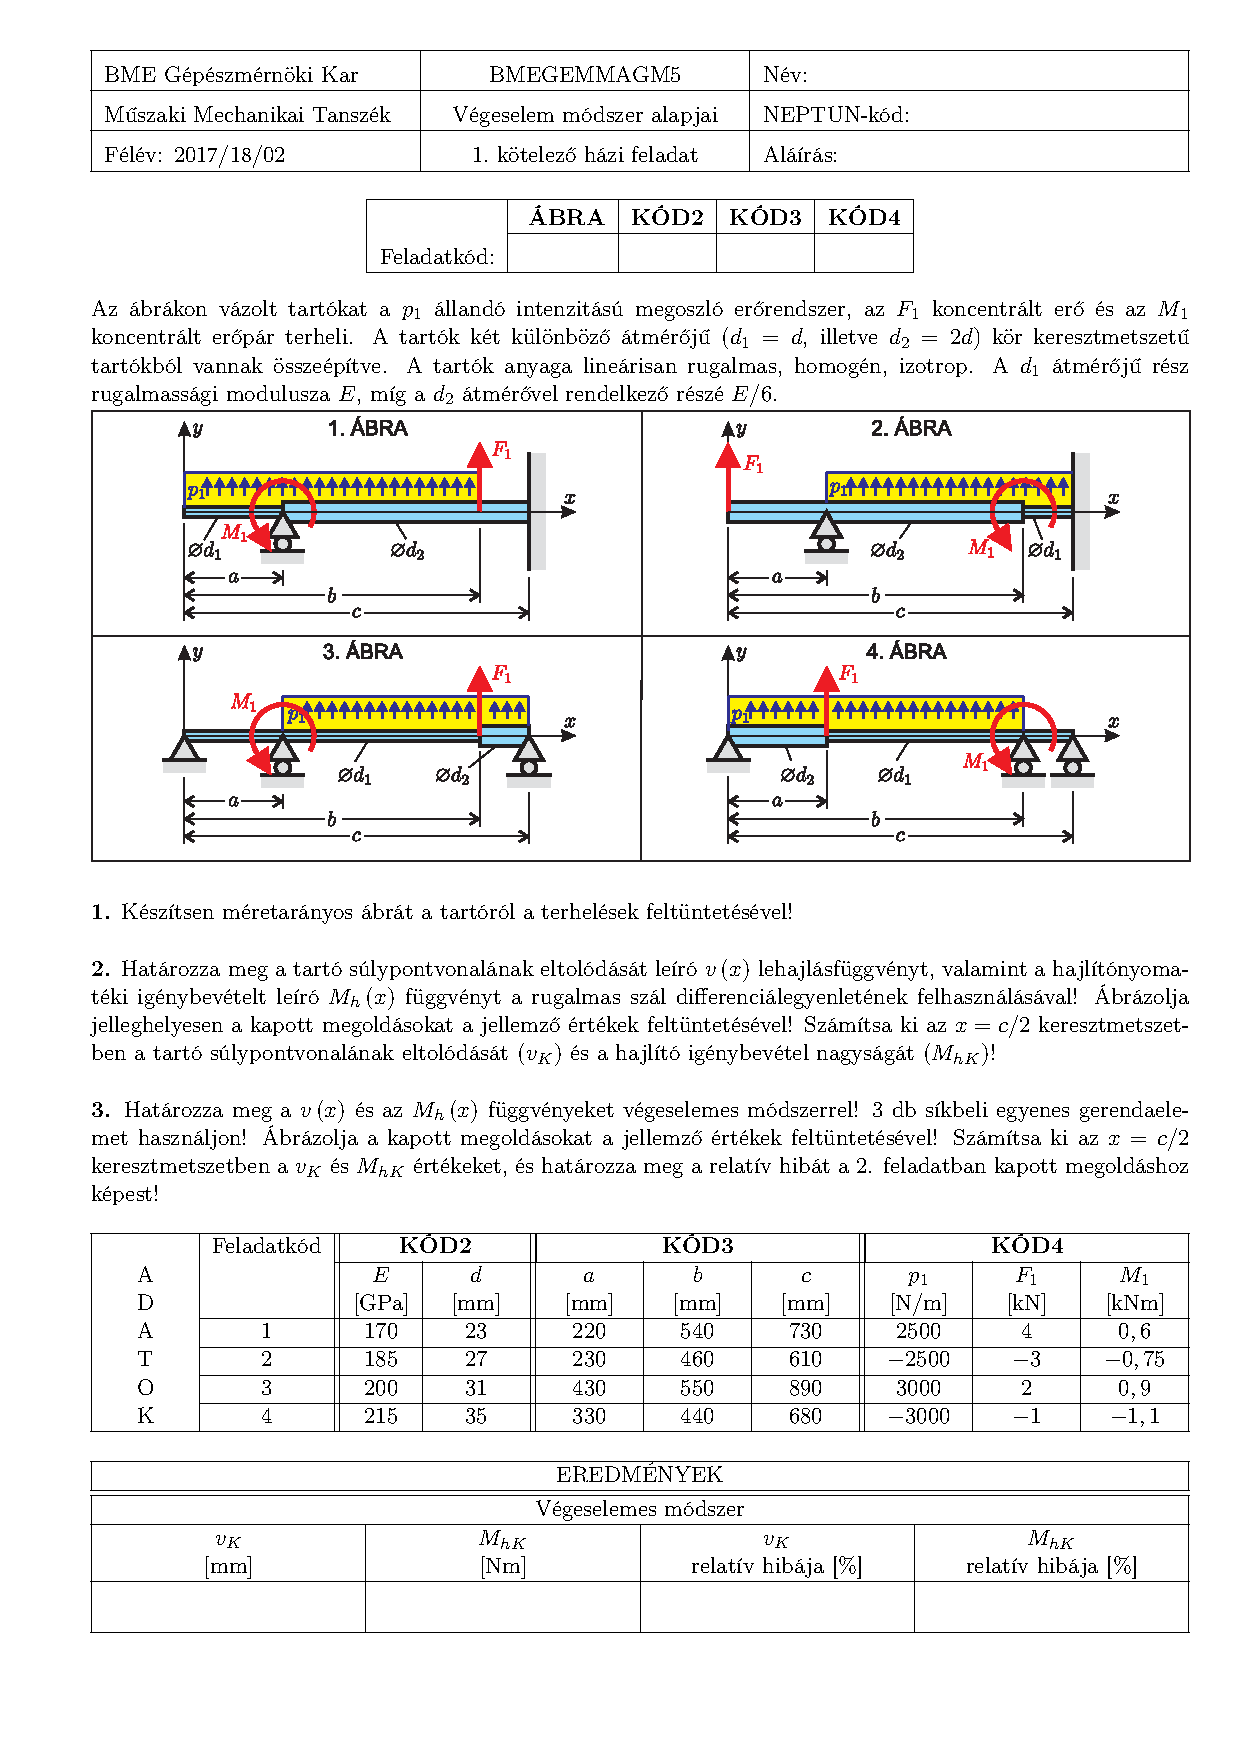
\includepdf[picturecommand*={
	    	\put(460,759){Tar Dániel}
	    	\put(460,740){GUTOY7}
	    	\put(280,677){2}
	    	\put(327,677){1}
	    	\put(370,677){2}
	    	\put(415,677){2}
	    	\put(115,63){eredmeny1}
	    	\put(245,63){eredmeny2}
	    	\put(370,63){eredmeny3}
	    	\put(490,63){eredmeny4}
	 }]{vemalaphf1.pdf}
	\newpage
	
	
	\setlength{\headheight}{0pt}
	\tableofcontents
	\newpage
	
	\pagenumbering{arabic}	
	\setcounter{page}{1}

	
	
	

	
	%\newpage
	
	\section{Feladat}
	
	A házifeladat kód alapján az adatokat átszámolva $[N][mm][MPa]$ alapra:
	
	\begin{table}[h!]
		\begin{center}
			\caption{Adatok}
			\label{tab:table1}
			\begin{tabular}{c|c|c|c|c|c|c|c|c} % <-- Alignments: 1st column left, 2nd middle and 3rd right, with vertical lines in between
				$E$ & $d_{1}$ & $d_{2}$ & $a$ & $b$ & $c$ & $p_{1}$ & $F_{1}$ & $M_{1}$ \\
				$[MPa]$ & $[mm]$ & $[mm]$ & $[mm]$ & $[mm]$ & $[mm]$ & $[N/mm]$ & $[N]$ & $[Nmm]$\\
				\hline
				$185\cdot10^3$ & 27 & 54 & 230 & 460 & 610 & -2.5 & -3000 & -0.75\\
				%2 & 10.1 & b\\
				%3 & 23.113231 & c\\
			\end{tabular}
		\end{center}
	\end{table}

	Az alapadatokból származtatott adatok:
	
	a1,a2,i1,i2
	
	\begin{flushleft}
		A terheléseket arányosan és mindenhol a pozitív irányba vettem fel, hogy megegyezzen a feladatleírásban szereplő ábrával.
	\end{flushleft}
	
	%\newcommand{\newCommandName}{text to insert}
	\newcommand{\degy}{8}
	\newcommand{\dketto}{16}
	
	\begin{figure}[h!]
		
		
		\begin{center}
			\begin{tikzpicture}
			\scaling{.015};
			
			% x and y axis
			\draw[->] (0,0)--(10,0) node[right]{$x$};
			\draw[->] (0,0)--(0,3) node[above]{$y$};
			
			% auxiliary points
			\point{a}{0}{0};
			\point{b}{230}{0};
			\point{c}{460}{0};
			\point{d}{610}{0};
			\point{e}{0}{\dketto}; %only to see it works :D
			\point{f}{0}{-\dketto};
			\point{g}{460}{\dketto};
			\point{h}{460}{-\dketto};
			\point{i}{460}{\degy};
			\point{j}{460}{-\degy};
			\point{k}{610}{\degy};
			\point{l}{610}{-\degy};
			
			
			\point{a2}{0}{78};
			\point{b2}{230}{53};
			\point{c2}{450}{-\dketto};
			\point{d2}{610}{53};
			
			% stucture
			\beam{2}{e}{f};
			\beam{2}{e}{g};
			\beam{2}{f}{h};
			\beam{2}{g}{h};
			\beam{2}{i}{k};
			\beam{2}{j}{l};
			
			%\support{type}{insertion point}[rotation];
			\support{2}{b};
			\support{3}{d}[90];
			
			% loads
			% \load{type}{insertion point}[rotation][length or included angle][loaddistance];
			\load{1}{a2}[90][-1];
			\load{3}{c}[25][200][0.7];
			\lineload{2}{b2}{d2}[-0.83][-0.83];
			
			% dimensions
			\dimensioning{1}{a}{b}{-1.2}[$230~mm$];
			\dimensioning{1}{a}{c}{-2.2}[$460~mm$];
			\dimensioning{1}{a}{d}{-3.2}[$610~mm$];
			%\dimensioning{2}{f}{e}{-1}[$54$];
			
			
			
			\notation{1}{a}{$A$}[left];
			\notation{1}{b}{$B$}[above left=2.5mm];
			\notation{1}{c}{$C$}[below right=2.5mm];
			\notation{1}{d}{$D$}[above right=2.5mm];
			
			\notation{1}{a2}{$F_{1}$}[right];
			\notation{1}{b2}{$p_{1}$}[below right];
			\notation{1}{c2}{$M_{1}$}[below=1mm];
			
			
			\end{tikzpicture}
		\end{center}	
		\caption{Méretarányos ábra és a terhelések}
	\end{figure}
	
	Rajz a rekcióerők feltüntetésével:
	rajz
	
	\newpage
		
	\section{Feladat - Rugalmas szál differenciálegyenlete}
		A rugalmas szál diffrenciálegyenletéhez a hajlítónyomatéki függvények felírása szükséges. A tartót 3 részre osztottam és mind a három tartományra felírhatam a hajlítónyomatéki függvényeket:
		
		hajlíto nyomatéki függvények..
		
		A rugalmas szál differenciálegyenlete a három tarományra:
		
		egyenletek...
		
		A differenciálegyenletek megoldásához illesztési feltételeket, kényszerfelételeket, illetve statikai egyensúlyt leíró egyenleteket is fel kell írni.
		
		Illesztési feltételek:
		....
		Kényszerek: 
		....
		Egyensúlyi egyenletek:
		....
		
		A rugalmas szál differenciálegyenleteiből a lehajlásfüggvényeket kétszeres integrálással kaphatjuk meg. Az integrálások miatt 6[db] ismeretlen értékű integrálási konstans jelenik meg. Ezen hat ismeretlenen kívül, ismeretlenek még a reakcióerők $(F_{By}, F_{Dx}, F_{Dy}, M_{D})$.
		
		Így egy tíz ismeretlenes egyenletrendszer áll elő, amelyekhez 10 peremfeltételt határoztunk meg. Ennek megfelelően az egyenletrendszerből az összes ismeretlen meghatározható.
		
		Számolt értékek:
		c-k, reakcioerok
		
		Ezek alapján az érékeket visszahelyettesítve a lehajlásfüggvényekbe:
		lehajlásfüggvények a szakaszokon
		
		plotok :
		szogelfordulás
		hajlítonyomateki
	
	
	\section{Feladat - Végeselemes megoldás}
		A feladat szövege alapján a végeselemes modell:
		vegeselemes modell (ábra) - 3 elem - 4 csomopont
		
		Elemi merevségi mátrix
		
		A 3[db] egyenes gerendaelem elemi merevségi mátrixait elhelyezzük a globális merevségi mátrixban a hozzájuk tarozó szabadsági fok összerendelések alapján.
		
		ábra - glob merev mátrix
		
		Ahol az általános elmozdulás és tehervektor:
		vektorok...
		
		A tehervektor a koncentrált erők és megoszló terhelések összegeként írható fel. A megoszló erőt a két rúdra külön felírva:
		koncentrált, megoszlo2, megoszlo3
		
		Az elmozdulásvektor megkötött paraméterei alapján kondenzáljuk a globális merevségi mátrixot úgy, hogy a merevségi mátrix oszlopait és sorait töröljük ott ahol az elmozdulásvektor nulla.
		
		A kondenzált merevségi mátrix:
		vektor...
		
		A kondenzált elmozdulásvektor:
		vektor...
		
		Az így alkotott $\textbf{K}_{kond}\cdot\textbf{U}_{kond}=\textbf{F}_{kond}$ egyenletrendszer megoldásával az elmozdulásvektor:
		elmozdulásvektor...
		
		A tehervektort pedig az elmozdulásvektor visszahelyettesítésével:
		tehervektor..
		
		A tehervektor komponenseiből kiolvashatóak a reakcióerők:
		rekcióerok...
		
		A végeselemes megoldás útján kapott eredmények szinte teljesen megegyeznek a rugalmas szál differenciál egyenletével számolt eredményekkel.
		
		
		
		
		
		
		
	
			
	
	
	

\end{document}
